% !TEX TS-program = pdflatex
% !TEX encoding = UTF-8 Unicode
%
% Aux .tex file to store some of the content of the mSystems paper to be moved
% to the complexCrucher specific paper that should be prepared once decided to
% detach CC in a different specific paper (probably targeting a bioinformatics
% journal) 
%

\subsection*{Specific results}

%%
\subsubsection*{Fit Plots}
For each and every dataset included in the study, an unweighted fit and a X-weighted fit (see Material and Methods section for details on both fits) have been calculated for standard deviations versus the mean values for each bacterial genus monitored in time. Figure \ref{fig:main1} showed the X-weighted fit for samples from a healthy subject (patient A, top) and from a subject diagnosed with irritable bowel syndrome (patient P2, bottom) studied in our lab\cite{IBS}, while Figure \ref{fig:fits} shows the corresponding unweighted fits. Both for the X-weighted and the unweighted fit, the IBS patient shows significative higher values of $V$ and $\beta$ than the healthy subject.

\begin{figure}
	\centering
	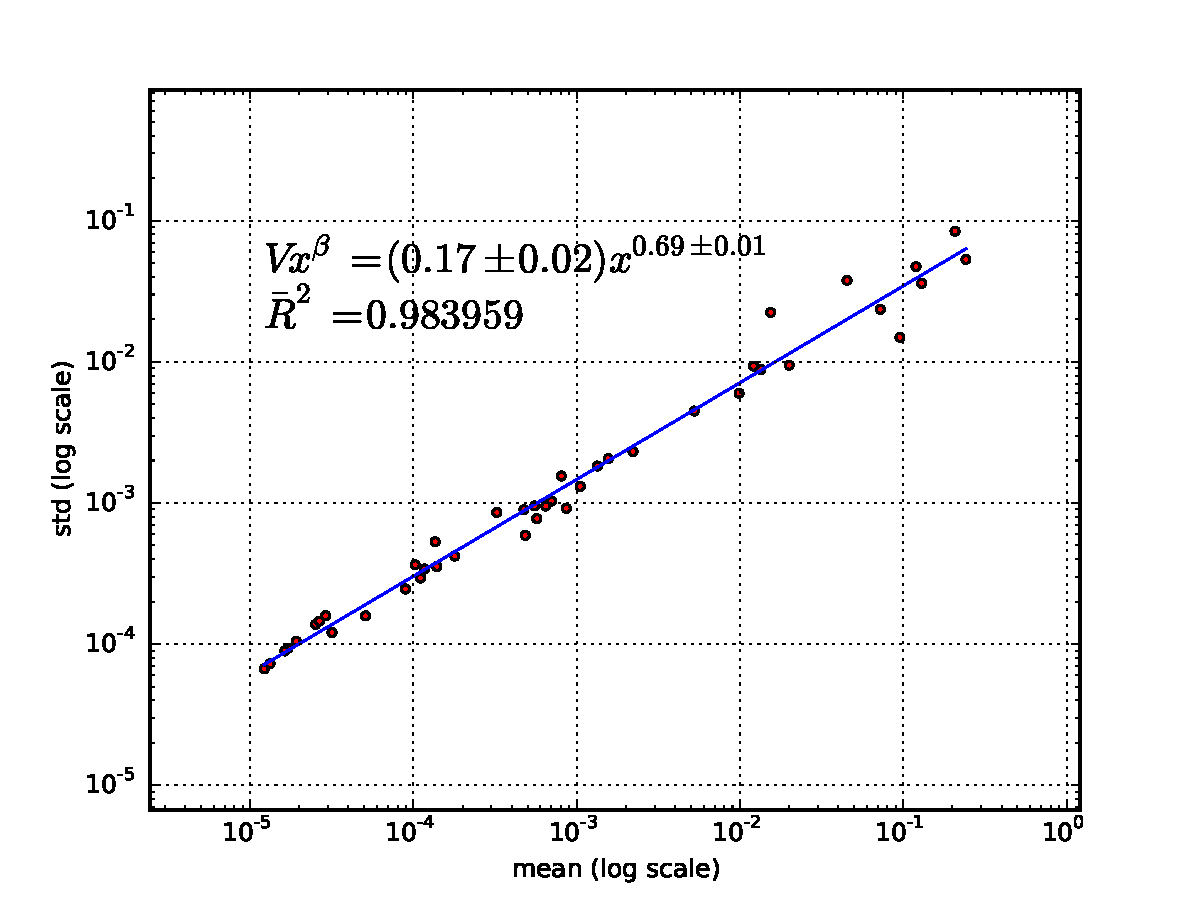
\includegraphics[width=0.8\textwidth]{results/fits/IBS_h_A_amplicons_family_stdVSmean_LLR_LOG.pdf}
	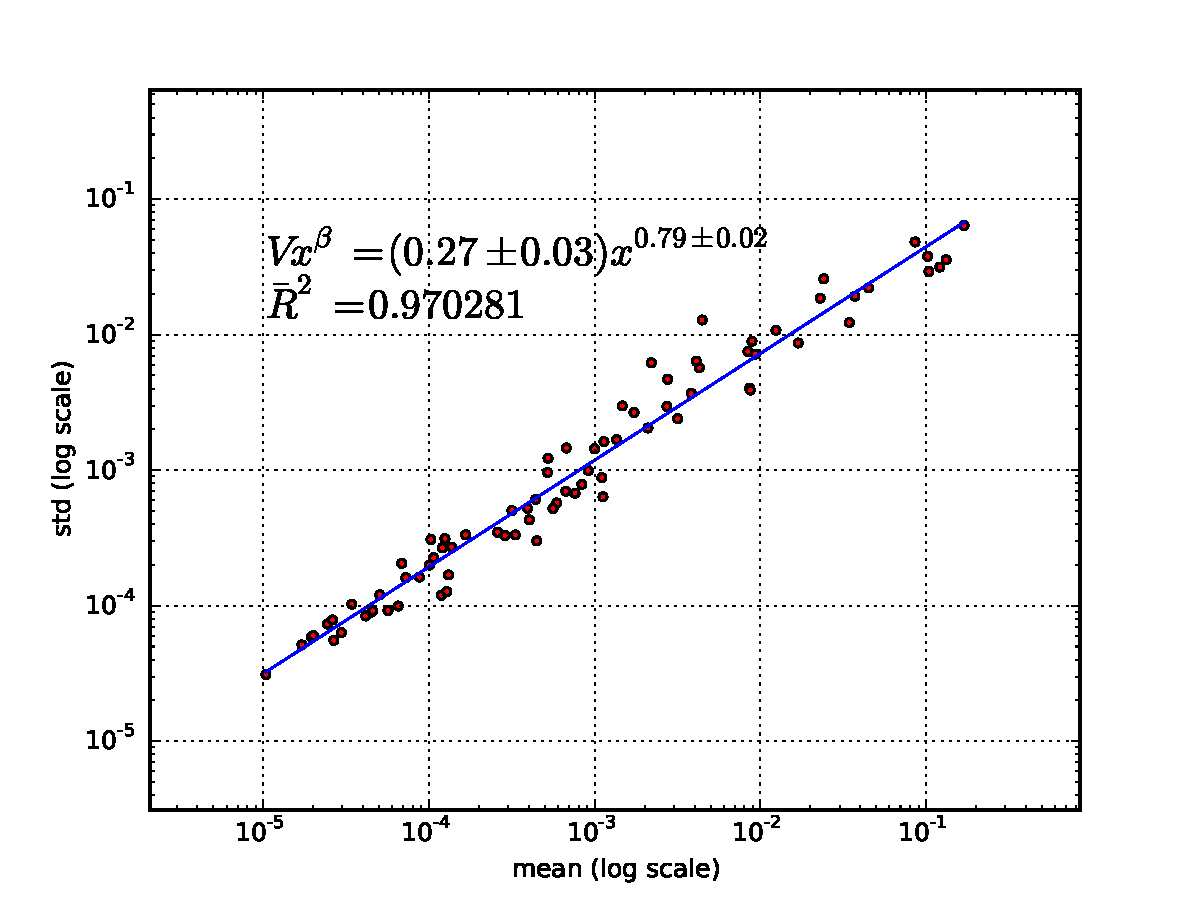
\includegraphics[width=0.8\textwidth]{results/fits/IBS_P1_metatranscriptomes_family_stdVSmean_LLR_LOG.pdf}
	\caption{Log plots of unweighted fits corresponding to the datasets shown in Figure \ref{fig:main1}, a healthy subject (top) and from a subject diagnosed with irritable bowel syndrome (bottom) studied in our lab \cite{IBS}}
	\label{fig:fits}
\end{figure}

Additionally, for the unweighted fit, a complete residues analysis was performed, and a 4-in-1 figure was generated as shown in Figure \ref{fig:unwRes}, corresponding to patient A (top plot in Figure \ref{fig:main1} and Figure \ref{fig:fits}). This allows to check for normality and homoscedasticity of the residues and, therefore, to further assess the goodness of the model's fit to the data.

\begin{figure}
	\centering
	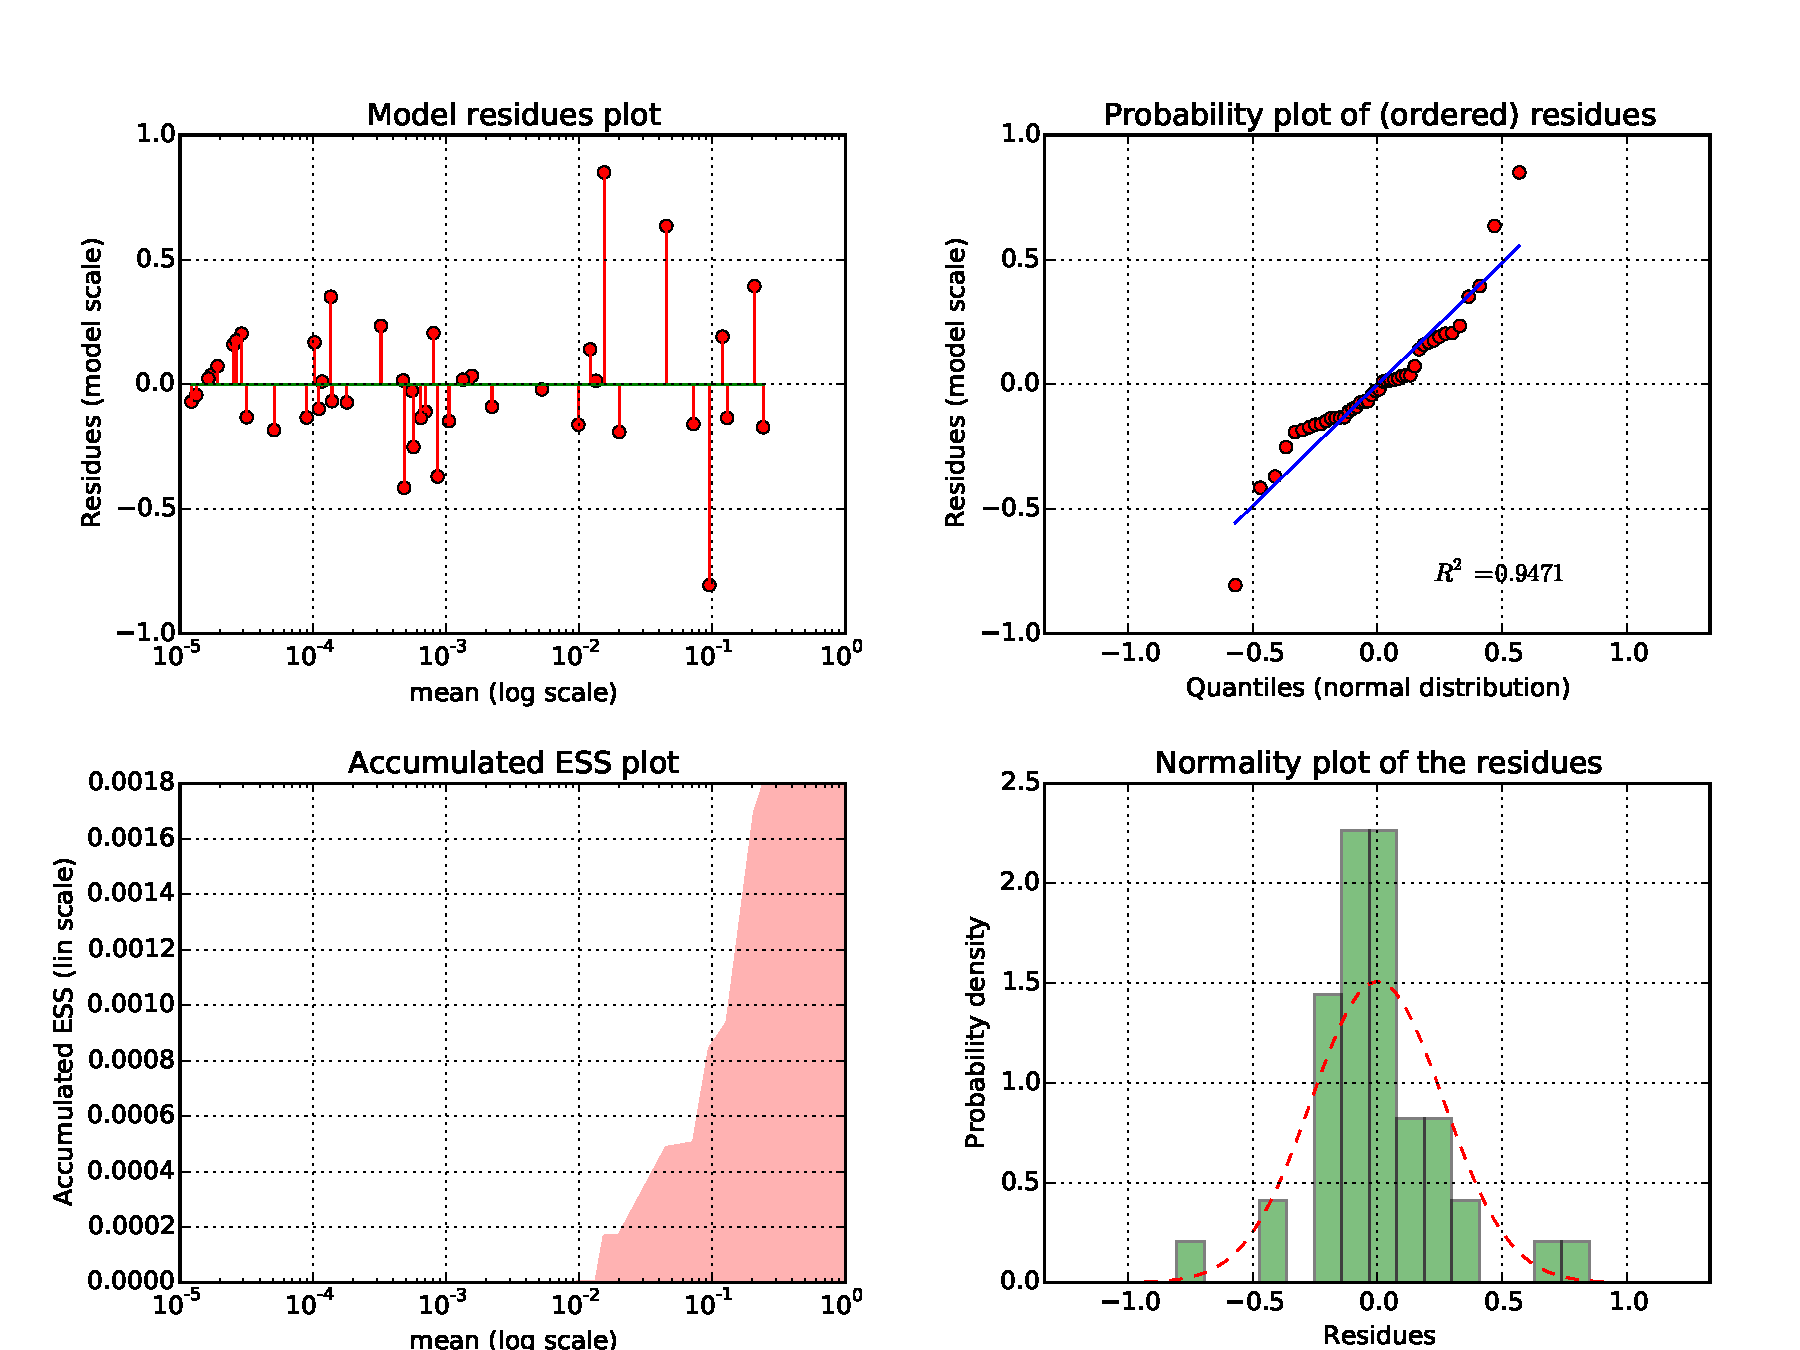
\includegraphics[width=\textwidth]{results/fits/IBS_h_A_amplicons_family_stdVSmean_LLR_RES.pdf}
	\caption{Residues analysis plot corresponding to the unweighted fit for patient A of the IBS study\cite{IBS}. The top-left subplot is a simple residues plot. The top-right subplot is a Normal quantiles plot with linear fitting (value of coefficient of determination is provided). The bottom-left subplot shows an accumulated ESS (Explained Sum of Squares) plot. Finally, the bottom-right subplot is a residues Normal histogram plot. This set of subplots allows to check for normality and homoscedasticity of the residues and, therefore, to further assess the goodness of the model's fit to the real data.}
	\label{fig:unwRes}
\end{figure}

\subsubsection*{Histogram Plots} 
The \CC\ software generates two related histogram plots: absolute frequencies plot and zero relative frequency plot. The former is useful to visually assess the validity of the time points in terms of the accumulated absolute frequency of the elements (taxa), since absolute frequencies far (much higher or much lower) from those typically observed could mean a sampling problem. In Figure \ref{fig:histAFP} shows this histogram for the pre-treatment data (first 7 times) of patient ``D'' in the antibiotics study\cite{antibiotic}. We can see that there are no \emph{outlayers} among the total taxa sum for the sample points of this time series, so all of them were considered for further analysis by \CC.

On the other hand, we could define the ZRF (Zero Relative Frequency, thereby ranging from 0 to 1) of an element (taxon) as the portion of times of the time series where the corresponding frequency is zero, i.e., such taxon is not found. The ZRF is useful for assessing how regularly is appearing the microbiota in the samples. In that sense, we define the ``core'' as the taxa that has a ZRF of less than 0.2, i.e., is present in more than the 80\% of the samples.

Attending to all taxa in a dataset, we can plot the ZRF histogram, which then lies on the horizontal axis of the plot, with the vertical axis showing the number of taxa. So, the height of a bar represents the amount of taxa that have determinate ZRF. In this respect, the bar near $0$ counts the quantity of taxa that are present at every (or almost every) time point of the data set. In the same way, in the opposite case, the bar near $1$ counts the total of taxa that are scarcely found but present at least in one time (the software filters any taxon not appearing at any time). Figure \ref{fig:histZRF} shows this plot for the healthy patient A of the IBS study performed in our lab\cite{IBS}. There, we can see that $12$ taxa are present at all the time points of the time series while $9$ taxa basically appear only once. Ranging between those extremes, there are a significative amount of elements, $23$ taxa, appearing from often to seldom, but not belonging to the ``core'' region.
	
\begin{figure}		
	\centering		
 	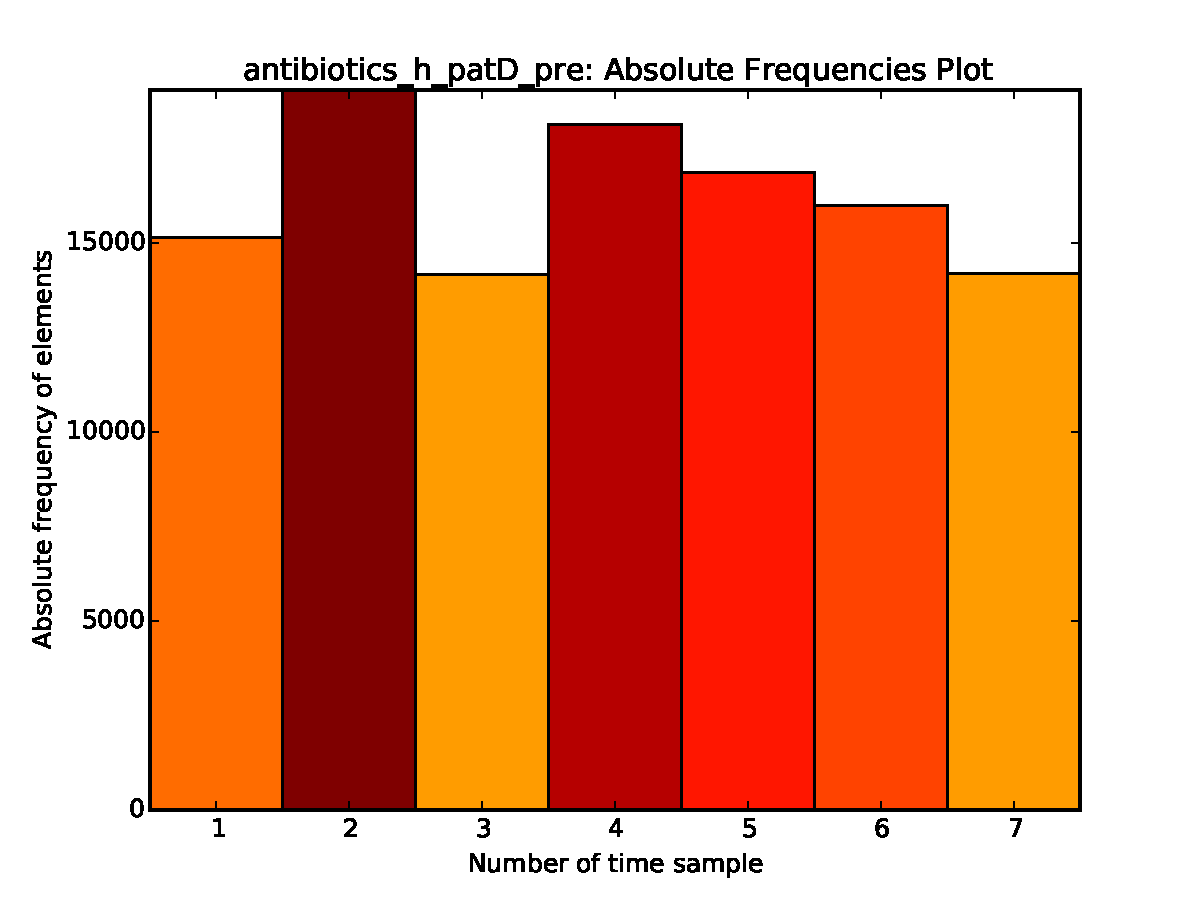
\includegraphics[width=0.8\textwidth]{results/hist/antibiotics_h_patD_pre_AbsFreqPlot}		
 	\caption{Histogram with the absolute frequencies of the pre-treatment data (7 first times) of patient ``D'' in the antibiotics study\cite{antibiotic}. There are no \emph{outlayers} among the total taxa sum for the time series sample points, so all of them were considered for further analysis by \CC\ software}		
 	\label{fig:histAFP}		
\end{figure}

\begin{figure}
	\centering
	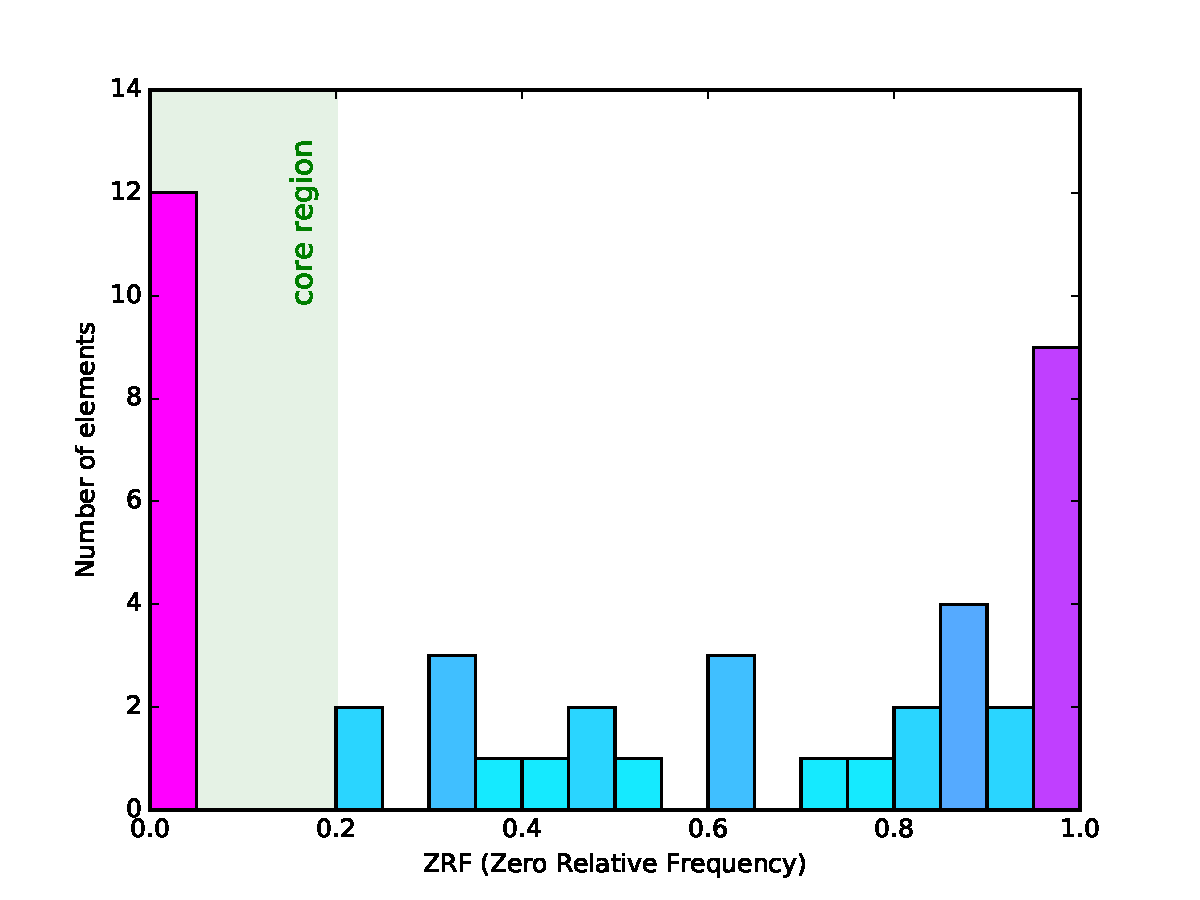
\includegraphics[width=0.8\textwidth]{results/hist/IBS_h_A_amplicons_family_ZRFhist.pdf}
	\caption{Histogram with the relative frequency of zero for the elements (taxa) in the data for patient A of the IBS study\cite{IBS}. In this particular case, the bar near $0$ counts the quantity of taxa that are present at almost every time point of the data set, while the bar near $1$ sums the total of taxa that are scarcely found: here, $12$ taxa are present at all the time points of the time series while $9$ taxa basically appear only once.}
	\label{fig:histZRF}
\end{figure}

A 2D semi-logarithmic histogram representing deviations from the mean versus the mean itself is a useful tool in the analysis of the stability of ranking processes in complex systems\cite{ranking}. Figure \ref{fig:hist2D} shows this 2D deviation plot for the patient A of the IBS study\cite{IBS}.
 
\begin{figure}
	\centering
	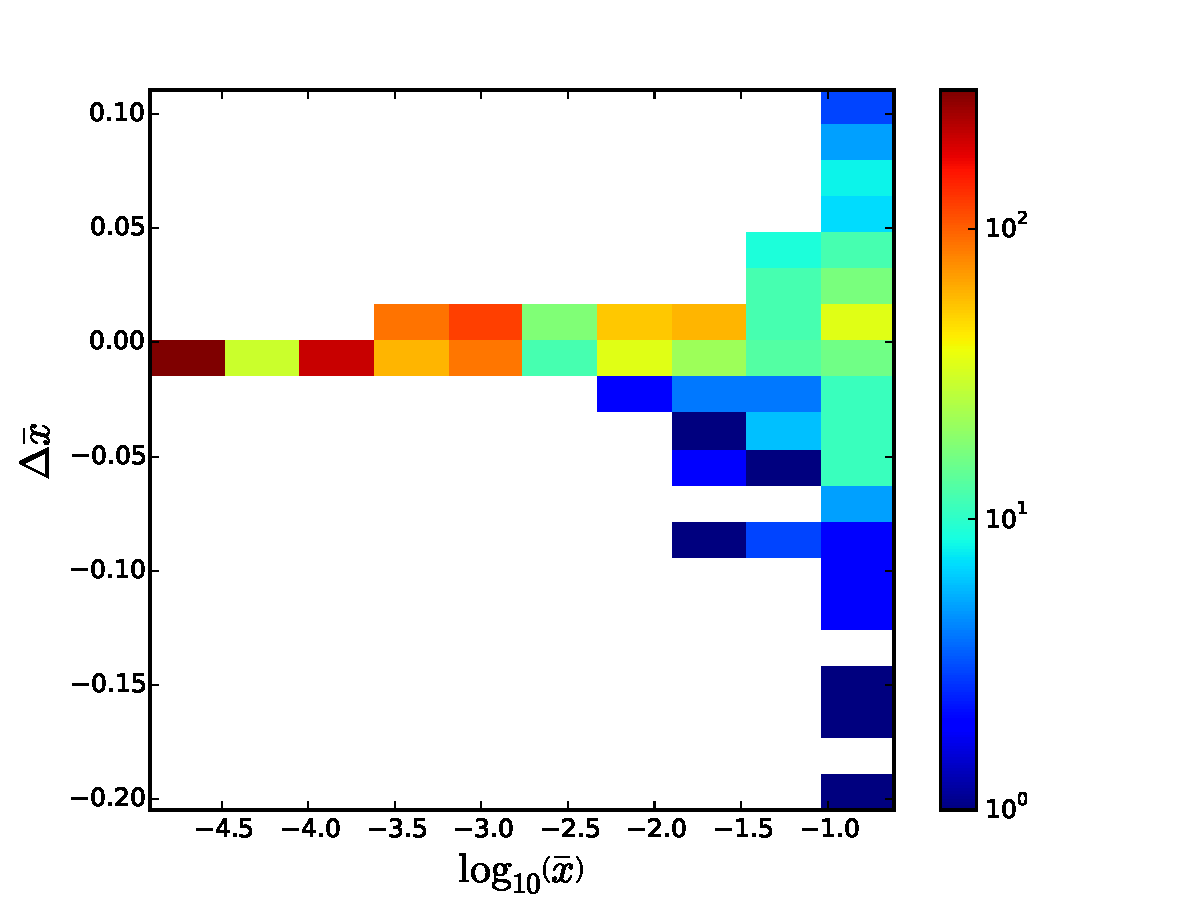
\includegraphics[width=0.8\textwidth]{results/hist/IBS_h_A_amplicons_family_hist2D.pdf}
	\caption{2D histogram deviation plot of the data for patient A of the IBS study\cite{IBS}}
	\label{fig:hist2D}
\end{figure}


%% Partial inclusion
\subsubsection*{Correlation and Rank Plots} 
\CC\ generates two different plots falling under this category in addition to the Excel files with the resulting matrices. On the one hand, the elements correlation matrix plot shows a correlation matrix among the taxa, calculated with the time as independent variable. For these calculations, the data set is not normalized to avoid entering an additional constraint. Figure \ref{fig:corrElm} shows this matrix for the most dominant taxa present in the data of the patient ``A'' of the IBS study\cite{IBS}. On the other hand, the rank dynamics and stability plot shows the variation in the rank with time for the most dominant taxa and their calculated RSI, as discussed in Material and Methods. Figure \ref{fig:corrank} shows this plot for the taxa of the aforementioned patient A.

\begin{figure}
	\centering
	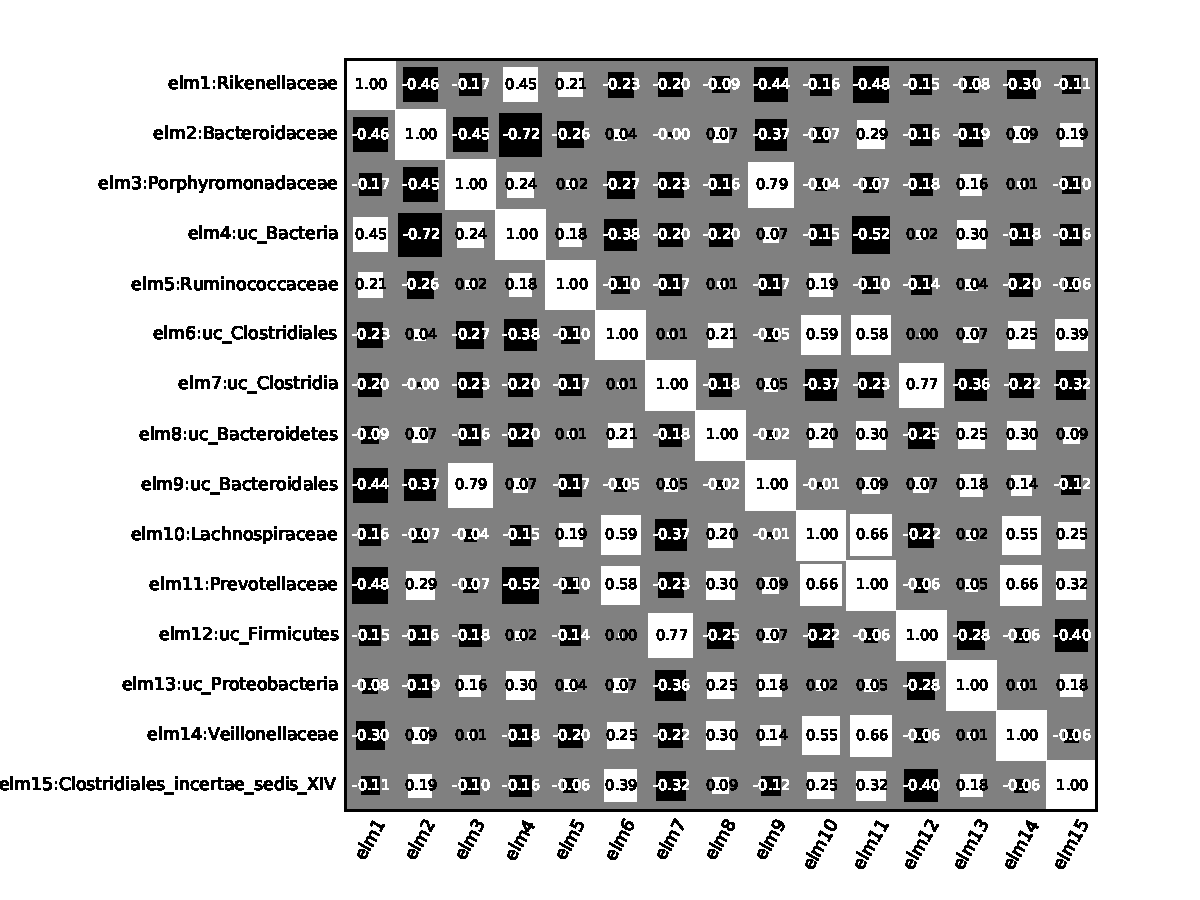
\includegraphics[width=0.9\textwidth]{results/corrank/IBS_h_A_amplicons_family_ElmCorrelation.pdf}
	\caption{Element correlation plot of the for the most dominant taxa in the data for patient A of the IBS study\cite{IBS}}
	\label{fig:corrElm}
\end{figure}

\begin{figure}
	\centering
	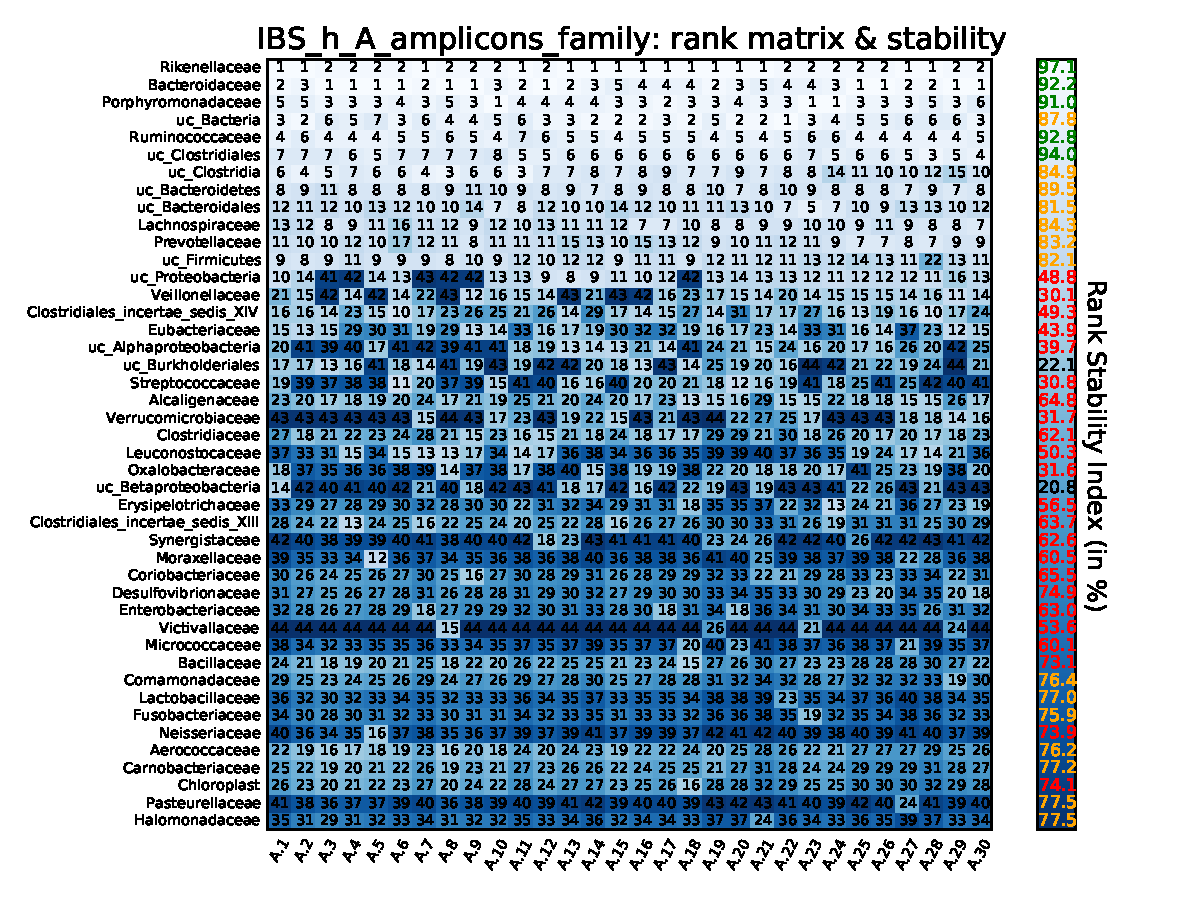
\includegraphics[width=\textwidth]{results/corrank/IBS_h_A_amplicons_family_Rank.pdf}
	\caption{Matrix showing the rank variation throughout time for the most dominant elements (taxa) and their calculated Rank Stability Index (as discussed in Material and Methods) in the data  for patient A of the IBS study\cite{IBS}}
	\label{fig:corrank}
\end{figure}

%%
\subsection*{ComplexCruncher}

A complete software framework, named 'ComplexCruncher', has been engineered to support the analysis of the dynamics of ranking processes in complex systems. Although the software was devised with a clear bias towards metagenomics, it is general enough to be able to cope with a ranking process in any complex system. Implemented in Python using well-known open-source community software, the software solution is composed of two parts that can be used together or apart: a web-based graphic front-end connected to a database, and a computing kernel. Used together, this software enables other users to reproduce our results easily and, furthermore, upload and analyse their own data or experiment with the preloaded metagenomics data sets.

`ComplexCruncher WebPortal' (CCWebPortal) is a web platform designed to allow the user to interact with a data repository of selected and well-documented metagenomics data sources. Through a few simple steps, the user can perform advanced searches on the complete set of records in the metagenomics repository.  The web application provides advanced filters that allow the user to reduce the search to a small set of interest. After this first step, the user can refine the search and discard those records that do not meet certain requirements.

The web application allows calculations to be done directly by the stable release of the \CC\ computing kernel. At the end of the calculations, the results are displayed to the user on the same browser which runs the web application. Then, the user can interact over the series of generated graphics thus allowing flexible comparison among them. In addition, CCWebPortal enables direct download of generated data (plots, spreadsheets, etc). The web application generates a report file summarizing all the results in PDF format. If the user has login permissions, CCWebPortal enables the option of insert new database records in addition to editing and deleting existing ones.

CCWebPortal is a web application that runs on current versions of many browsers. Additional software is not needed and only requires javaScript to be enabled on the browser to run applications. 
CCWebPortal is implemented following the client$-$server distributed programming model, where the javaScript client application connects to a remote server that enables the execution of calculations and transactions through a centralized database management system. A set of relational tables allows the structuring of the metagenomics repository to establish relationships between records. Thus the search and information threshing is optimized for queries launched from the client interface. Access to the database on the server is implemented through Django framework, an open-source framework written in Python using the model-view-controller (MVC) architectural pattern for implementing user interfaces.

The effective data analysis has been performed with a Python tool developed from scratch to more than 4200 lines of code. Implemented following the Object Oriented Programming paradigm, this software is the back-end of the website described above. However, it could be run as an independent piece of software since it is built as a Python package provided with a command-line front-end (\CC.py). Once installed, the tool can be run interactively but also in automatic mode, which uses parallel computation to speed up the analysis of several data sources. 

\CC\ performs the power-law fit described in the \emph{Blumm, N. et al.} paper, but by fitting the best model, i.e. choosing between fitting a power-law using linear regression versus nonlinear regression\cite{ecology}. In the power-law fit plots we also show the generalized coefficient of determination computed for continuous models\cite{genR2,disR2}.

%%
\subsection*{Un-weighted power-law fit}\label{sec:unw}

\subsubsection*{Fitting the best model}

As already mentioned, to choose between fitting power laws ($y=Vx^\beta$) using linear regression on log-transformed (LLR) data versus non-linear regression (NLR), we mainly follow \emph{General Guidelines for the Analysis of Biological Power Laws}\cite{ecology}. It consists of the following three steps:
\begin{enumerate}
    \item Determining the appropriate error structure by likelihood analysis.
    \begin{enumerate}
        \item Fit the Non-Linear Regression (NLR) model and obtain $V_\text{NLR}$, $\beta_\text{NLR}$ and $\sigma_\text{NLR}^2$.
        \item Calculate the loglikelihood that the data ($n$ is sample size) are generated from a normal distribution with additive error:
        \begin{itemize}
            \item The likelihood of a normal distribution is: 
            \begin{linenomath}
            $$\mathcal{L}_\text{norm} = \prod_{i=1}^n\left[\frac{1}{\sqrt{2\pi\sigma^2_\text{NLR}}}\;\exp{\left(-\frac{\left(y_i-V_\text{NLR}x_i^{\beta_\text{NLR}}\right)^2}{2\sigma^2_\text{NLR}}\right)}\right]$$
            \end{linenomath}
            \item So, the loglikelihood of a normal distribution is:
            \begin{eqnarray*}
                \log\mathcal{L}_\text{norm} &=& -\frac{n}{2}\log\left|2\pi\sigma^2_\text{NLR}\right| - \frac{1}{2\sigma^2_\text{NLR}}\underbrace{\sum_{i=1}^n\left(y_i-V_\text{NLR}x_i^{\beta_\text{NLR}}\right)^2}_{\mathrm{RSS
                }_\text{NLR}}\\
                &=& -\frac{n}{2}\log\left|2\pi\sigma^2_\text{NLR}\right|-\frac{\mathrm{RSS}_\text{NLR}}{2\sigma^2_\text{NLR}}
            \end{eqnarray*}
        \end{itemize}
        \item Calculate the \emph{corrected Akaike's Information Criterion} for the NLR model:
		\begin{linenomath}
        $$\mathrm{AIC_{c_{NLR}}} = 2k - 2\log\mathcal{L}_\text{norm} + \frac{2k(k+1)}{n-k-1}$$
		\end{linenomath}
        \item Fit the Log-transformed Linear Regression (LLR) model and obtain $V_\text{LLR}$, $\beta_\text{LLR}$ and $\sigma_\text{LLR}^2$.
        \item Calculate the loglikelihood that the data ($n$ is sample size) are generated from a lognormal distribution with multiplicative error:
        \begin{itemize}
            \item The likelihood of a lognormal distribution is: 
            \begin{linenomath}
            $$\mathcal{L}_\text{logn} = \prod_{i=1}^n\left[\frac{1}{y_i\sqrt{2\pi\sigma^2_\text{LLR}}}\;\exp{\left(-\frac{\left(\log|y_i|-\log|V_\text{LLR}|-\beta_\text{LLR}\log|x_i|\right)^2}{2\sigma^2_\text{LLR}}\right)}\right]$$
            \end{linenomath}
            \item So, the loglikelihood of a lognormal distribution is: 
            \begin{eqnarray*}
                \log\mathcal{L}_\text{logn} &=& -\frac{n}{2}\log\left|2\pi\sigma^2_\text{LLR}\right| - \sum_{i=1}^n\log|y_i| -\\
                &&\qquad-\frac{1}{2\sigma^2_\text{LLR}}\underbrace{\sum_{i=1}^n\left(\log|y_i|-\log|V_\text{LLR}|-\beta_\text{LLR}\log|x_i|\right)^2}_{\mathrm{RSS
                }_\text{LLR}}\\
                &=& -\frac{n}{2}\log\left|2\pi\sigma^2_\text{LLR}\right| - \frac{\mathrm{RSS}_\text{LLR}}{2\sigma^2_\text{LLR}} - \sum_{i=1}^n\log|y_i|
            \end{eqnarray*}
        \end{itemize}
        \item Calculate the \emph{corrected Akaike's Information Criterion} for the LR model: 
        	\begin{linenomath}
        	$$\mathrm{AIC_{c_{LLR}}} = 2k - 2\log\mathcal{L}_\text{logn} + \frac{2k(k+1)}{n-k-1}$$
			\end{linenomath}
    \end{enumerate}
    \item Compare $\mathrm{AIC_{c_{NLR}}}$ with $\mathrm{AIC_{c_{LLR}}}$:
    \begin{itemize}
        \item If $\mathrm{AIC_{c_{NLR}}} - \mathrm{AIC_{c_{LLR}}} < -2$, the assumption of normal error is favoured compared to lognormal error, so proceed with the results obtained from the NLR fit.
        \item If $\mathrm{AIC_{c_{NLR}}} - \mathrm{AIC_{c_{LLR}}} > 2$, the assumption of lognormal error is favoured compared to normal error, so proceed with the results obtained from the LLR fit.
        \item If $\left|\mathrm{AIC_{c_{NLR}}} - \mathrm{AIC_{c_{LLR}}}\right| \leq 2$, no model is favoured, so proceed with model averaging:
        \begin{eqnarray*}
            B_\text{av} &=& w_\text{NLR}V_\text{NLR} + w_\text{LLR}V_\text{LLR} \\
            \beta_\text{av} &=& w_\text{NLR}\beta_\text{NLR} + w_\text{LLR}\beta_\text{LLR}
        \end{eqnarray*}
        where: 
        \begin{eqnarray*}
            w_\text{NLR} &=& \frac{1}{1+\mathrm{e}^{\frac{1}{2}\left(\mathrm{AIC_{c_{NLR}}}-\mathrm{AIC_{c_{LLR}}}\right)}} \\
            w_\text{LLR} &=& \frac{1}{1+\mathrm{e}^{\frac{1}{2}\left(\mathrm{AIC_{c_{LLR}}}-\mathrm{AIC_{c_{NLR}}}\right)}}
        \end{eqnarray*}
        which are obtained to fulfill the next condition: $w_\text{NLR} + w_\text{LLR} = 1$. The CIs for $B_\text{av}$ and $\beta_\text{av}$ are to be generated by ordinary bootstrapping\footnote{\CC\ has available the next bootstrapping alternatives\cite{boot}: ordinary, ``Resampling Residuals'' method, ``Wild'' method, and ``Monte-Carlo'' method.}.      
    \end{itemize}
    \item Assess the validity of the underlying statistical assumptions with diagnostic plots because while it is rare for all the assumptions to be fully satisfied by real-life data sets, major violations indicate the lack of appropriateness of the model and, thus, the potential invalidity of the results.
\end{enumerate}

\subsubsection*{Calculating the coefficient of determination}

We think the best approach in this situation is to apply the generalized $R^2$ that, for continuous models, was defined as\cite{genR2}:
\begin{linenomath}
$$ R^2 = 1 - \left(\frac{\mathcal{L}(0)}{\mathcal{L}(\hat\theta)}\right)^{\!\!\frac{2}{n}} $$
\end{linenomath}
where $\mathcal{L}(\hat\theta)$ and $\mathcal{L}(0)$  denote the likelihoods of the fitted and the ``null'' model, respectively, and $n$ is the sample size. In terms of the loglikelihoods, the generalized coefficient of determination would be:
\begin{linenomath}
$$ R^2 = 1 - \mathrm{e}^{-\frac{2}{n}\left(\log\mathcal{L}(\hat\theta)-\log\mathcal{L}(0)\right)} $$
\end{linenomath}
We have the likelihoods calculated from the previous section, but what about the ``null'' models? We understand that they are the models with only the intercept. So for the Gaussian additive error model:
\begin{linenomath}
$$\mathcal{L}_\text{norm}(0) = \prod_{i=1}^n\left[\frac{1}{\sqrt{2\pi\sigma^2_\text{NLR0}}}\;\exp{\left(-\frac{\left(y_i-\bar y\right)^2}{2\sigma^2_\text{NLR0}}\right)}\right]$$
\end{linenomath}
So:
\begin{eqnarray*}
\log\mathcal{L}_\text{norm}(0) &=& -\frac{n}{2}\log\left|2\pi\sigma^2_\text{NLR0}\right| - \frac{1}{2\sigma^2_\text{NLR0}}\sum_{i=1}^n\left(y_i-\bar y\right)^2\\
 &=& -\frac{n}{2}\left(\log\left|2\pi\sigma^2_\text{NLR0}\right| + 1 \right)
\end{eqnarray*}
since $\sigma^2_\text{NLR0}=\frac{1}{n}\sum\left(y_i-\bar y\right)^2=\frac{1}{n}\mathrm{TSS}_\text{NLR}$. Now, coming back to the coefficient of determination, we have:
\begin{eqnarray*}
R^2_\text{NLR} &=& 1 - \mathrm{e}^{\frac{2}{n}\left(\log\mathcal{L}_\text{NLR}(0)-\log\mathcal{L}_\text{NLR}(\hat\theta)\right)} = 1 - \exp{\left(\frac{\log(\mathrm{RSS}_\text{NLR})}{\log(\mathrm{TSS}_\text{NLR})}\right)}
 =\\ &=& 1 - \frac{\mathrm{RSS}_\text{NLR}}{\mathrm{TSS}_\text{NLR}} =
 1 - \frac{\sum_{i=1}^n\left(y_i-V_\text{NLR}x_i^{\beta_\text{NLR}}\right)^2}{\sum_{i=1}^n\left(y_i-\bar y\right)^2}
\end{eqnarray*}
recovering the traditional expression for $R^2$. Using the same approach for calculating $R^2_\text{LLR}$, then:
\begin{linenomath}
$$\mathcal{L}_\text{logn}(0) = \prod_{i=1}^n\left[\frac{1}{y_i\sqrt{2\pi\sigma^2_\text{LLR0}}}\;\exp{\left(-\frac{\left(\log|y_i|-\log|B_\text{LLR0}|\right)^2}{2\sigma^2_\text{LLR0}}\right)}\right]$$
\end{linenomath}
So:
\begin{eqnarray*}
\log\mathcal{L}_\text{logn}(0) &=& -\frac{n}{2}\log\left|2\pi\sigma^2_\text{LLR0}\right| - \frac{1}{2\sigma^2_\text{LLR0}}\sum_{i=1}^n\left(\log|y_i|-\overline{\log|y|}\right)^2 - \sum_{i=1}^n\log|y_i|\\
 &=& -\frac{n}{2}\left(\log\left|2\pi\sigma^2_\text{LLR0}\right| + 1 \right) - \sum_{i=1}^n\log|y_i|
\end{eqnarray*}
since $\sigma^2_\text{LLR0}=\frac{1}{n}\sum\left(\log|y_i|-\overline{\log|y|}\right)^2=\frac{1}{n}\mathrm{TSS}_\text{logn}$. Again, recalling the expression for the generalized coefficient of determination, we have:
\begin{eqnarray*}
R^2_\text{LLR} &=& 1 - \mathrm{e}^{\frac{2}{n}\left(\log\mathcal{L}_\text{LLR}(0)-\log\mathcal{L}_\text{LLR}(\hat\theta)\right)} = 1 - \exp{\left(\frac{\log(\mathrm{RSS}_\text{LLR})}{\log(\mathrm{TSS}_\text{LLR})}\right)}
 =\\ &=& 1 - \frac{\mathrm{RSS}_\text{LLR}}{\mathrm{TSS}_\text{LLR}} =
 1 - \frac{\sum_{i=1}^n\left(\log|y_i|-\log|V_\text{LLR}|-\beta_\text{LLR}\log|x_i|\right)^2}{\sum_{i=1}^n\left(\log|y_i|-\overline{\log|y|}\right)^2}
\end{eqnarray*}


%% Partially included
\subsection*{X-weighted power-law fit}\label{sec:X-w}

When fitting the power-law of std vs. mean, we can take into account that every mean has uncertainty and estimate it for a sample size $n$ by the SEM (\emph{Standard Error of the Mean}):
\begin{linenomath}
$$ \mathrm{SEM} = \frac{s}{\sqrt{n}}$$
\end{linenomath}
where $s$ is the sample standard deviation. So, the vector of weights is computed with:
\begin{linenomath}
$$ \mathbf{w} = \frac{1}{\overrightarrow{\mathrm{SEM}}} = \frac{\sqrt{\mathbf{n}}}{\mathbf{s}}$$
\end{linenomath}

Here, the uncertainties affect the independent variable, so the fit is not so trivial as a Y-weighted fit, where the uncertainties affect the dependent variable. A standard approach to do this fit is: a) invert your variables before applying the weights, b) then perform the weighted fit, and finally, c) revert the inversion. This method is deterministic, but the approximate solution worsens with smaller $R^2$. For comparison, we develop a stochastic method by using a bootstrapping-like strategy that avoids the inversion and is applicable regardless of $R^2$. Both methods, detailed below, are implemented in \CC.


%% Omitted
\subsubsection*{Method 1: By inverting the data}

In the case of the log-LR model, we have:
\begin{linenomath}
$$\log y = \log V + \beta\log x \quad\rightarrow\quad \underbrace{\log x}_{\tilde y} = \overbrace{-\frac{1}{\beta}\log V}^{b} + \overbrace{\frac{1}{\beta}}^{m}\underbrace{\log y}_{\tilde x}$$ 
\end{linenomath}
where $m$ determines the slope or gradient of the fitted line, and $b$ determines the point at which the line crosses the y-axis, otherwise known as the y-intercept. Once the model is fitted, the original parameters can be retrieved easily:
\begin{eqnarray*}
\beta &=& \frac{1}{m} \\
V &=& \mathrm{e}^{-\beta b} = \mathrm{e}^{-\frac{b}{m}}
\end{eqnarray*}
Their respective uncertainties are to be obtained using \emph{error propagation}:
\begin{eqnarray*}
    \sigma_\beta &=& \left|\frac{\mathrm{d}\beta}{\mathrm{d}m}\right|\sigma_m \quad=\quad \frac{1}{m^2}\;\sigma_m \\
    \sigma_V &=& \sqrt{\left(\frac{\partial V}{\partial b}\right)^{\!\!2}\sigma_b^2 +
      \left(\frac{\partial V}{\partial m}\right)^{\!\!2}\sigma_m^2} \quad=\quad
      \frac{1}{m}\;\mathrm{e}^{-\frac{b}{m}}\,\sqrt{\sigma_b^2 + \frac{b^2}{m^2}\;\sigma_m^2} 
\end{eqnarray*}

%% Partially included
\subsubsection*{Method 2: Bootstrapping-like strategy}

The basic idea of bootstrapping is that inference about a population from sample data (sample $\rightarrow$ population) can be modeled by resampling the sample data and performing inference on (resample $\rightarrow$ sample). To adapt this general idea to our problem, we resample the x-data array using its errors array. That is, for each replicate, a new x-data array is computed based on:
\begin{linenomath}
$$x^*_i = x_i + v_i$$
\end{linenomath}
where $v_i$ is a Gaussian random variable with mean $\mu_i=0$ and standard deviation $\sigma_i=\mathrm{SEM}_i$, as defined previously. For each replicate a complete un-weighted power-law fit is performed, as described in the previous section. It is worth mentioning that each replicate is filtered to avoid values of $x^*_i$ under \emph{eps} (obtained by \texttt{np.finfo(np.double).eps}) in order to keep away from the error of getting log of negatives or zero during the fit.

We devised and implemented a multi-step algorithm to estimate the fit parameters that finishes when a relative error of less than $10^{-4}$ is achieved. It also ends if the number of steps reaches $100$ to avoid too much time lapse, to prevent any pathologic numeric case which, in fact, we still have not detected in all the data sets analyzed.

In the previous version of the algorithm, for each step, the method generated $10$ replicates for each x-data point, in other words, it was computing the fit for $10$ times the length of the x-data array replicates, with a maximum of $10000$ fits per step. Nevertheless, we found that such an approach depending on the length of the x-data array did not perform better, so we decided to simplify the method and fix the number of fits per step in $100$. This latter approach improved the performance. 

The parameters of the X-weighted fit are then estimated by averaging through all the replicate fits performed, and their errors are estimated by computing the standard deviation also for all the fits. At the end of each step, the relative error is calculated by comparing the fit parameters estimation in the last step with the previous one.

Finally, both the coefficient of determination of the fit and the coefficient of correlation between the fit parameters are estimated by averaging.

%% Mostly included
\subsection*{Rank Stability Index (RSI)}\label{sec:RSI}

The Rank Stability Index is shown as a percentage in a separate bar on the right of the rank matrix plot provided by \CC. The RSI is strictly $1$ for an element whose range never changes over time, and is strictly $0$ for an element whose rank oscillates between the extremes from time to time. So, RSI is calculated, per element, as $1$ less the quotient of the number of true rank hops taken between the number of maximum possible rank hops, all powered to $p$:
\begin{linenomath}
$${\rm RSI} = \left(1-\frac{\text{true rank hops}}{\text{possible rank hops}}\right)^p = \left(1-\frac{D}{(N-1)(t-1)}\right)^p$$
\end{linenomath}
where $D$ is the total of rank hops taken by the studied element, $N$ is the number of elements that have been ranked, and $t$ is the number of time samples. The power index $p$ is arbitrarily chosen to increase the resolution in the stable region; the value in the current version of the code is $p=4$. 

As an example of this ``zooming'' effect in the stable region, to match a linear ($p=1$) RSI of 0.9 to a powered one of 0.1, we should select $p=21.8543$. An alternative way to obtain this effect and exactly map a linear RSI of 0.9 to a non-linear RSI (${\rm RSI'}$) of 0.1, is by applying the following function:
\begin{linenomath}
$${\rm RSI'} = \frac{10^{10\left(1-\frac{D}{(N-1)(t-1)}\right)}-1}{10^{10}-1} \approx 10^{-10\left(\frac{D}{(N-1)(t-1)}\right)}$$
\end{linenomath}
where the approximation is valid because $10^{10}\gg 1$ but, the small price to pay for it is that, in the worst instability case, the ${\rm RSI'}$ would not be strictly $0$ but $10^{-10}$.

The colour code of the RSI percentage text in the rank plot of \CC\ is chosen following the first condition satisfied from those shown in Table \ref{tab:RSI} (see page \pageref{tab:RSI}). 

\begin{table}
  \begin{center}
    \begin{tabular}{cccr}
    \hline
    Case  &  Condition  &  Colour  &  Description \\
    \hline
    1  &  $1\ge{\rm RSI}>0.99$  & \textcolor{blue}{blue} & constant rank \\ 
    2  & ${\rm RSI}>0.90$  &  \textcolor{green}{green}  & highly stable rank \\
    3  &  ${\rm RSI}>0.75$  &  \textcolor{orange}{orange} & moderately stable rank \\
    4  &  ${\rm RSI}>0.25$  &  \textcolor{red}{red} & unstable rank \\
    5  &  $0.25\ge{\rm RSI}\ge0$  &  \bfseries{black} & very unstable rank \\
    \hline
    \end{tabular}
  \end{center} 
  \caption{Colour code of the RSI percentage text shown in Figure \ref{fig:corrank}, following the first condition satisfied.}
  \label{tab:RSI}
\end{table}



